
\documentclass[a4paper,11.5pt]{article}
\usepackage[textwidth=170mm, textheight=230mm, inner=20mm, top=20mm, bottom=30mm]{geometry}
\usepackage[normalem]{ulem}
\usepackage[utf8]{inputenc}
\usepackage[T1]{fontenc}
\PassOptionsToPackage{defaults=hu-min}{magyar.ldf}
\usepackage{pgfplots}
\pgfplotsset{compat=1.10}
\usepgfplotslibrary{fillbetween}
\usepackage[magyar]{babel}
\usepackage{amsmath, amsthm,amssymb,paralist,array, ellipsis, graphicx, float, bigints,tikz}
%\usepackage{marvosym}

\makeatletter
\renewcommand*{\mathellipsis}{%
	\mathinner{%
		\kern\ellipsisbeforegap%
		{\ldotp}\kern\ellipsisgap
		{\ldotp}\kern\ellipsisgap%
		{\ldotp}\kern\ellipsisaftergap%
	}%
}
\renewcommand*{\dotsb@}{%
	\mathinner{%
		\kern\ellipsisbeforegap%
		{\cdotp}\kern\ellipsisgap%
		{\cdotp}\kern\ellipsisgap%
		{\cdotp}\kern\ellipsisaftergap%
	}%
}
\renewcommand*{\@cdots}{%
	\mathinner{%
		\kern\ellipsisbeforegap%
		{\cdotp}\kern\ellipsisgap%
		{\cdotp}\kern\ellipsisgap%
		{\cdotp}\kern\ellipsisaftergap%
	}%
}
\renewcommand*{\ellipsis@default}{%
	\ellipsis@before
	\kern\ellipsisbeforegap
	.\kern\ellipsisgap
	.\kern\ellipsisgap
	.\kern\ellipsisgap
	\ellipsis@after\relax}
\renewcommand*{\ellipsis@centered}{%
	\ellipsis@before
	\kern\ellipsisbeforegap
	.\kern\ellipsisgap
	.\kern\ellipsisgap
	.\kern\ellipsisaftergap
	\ellipsis@after\relax}
\AtBeginDocument{%
	\DeclareRobustCommand*{\dots}{%
		\ifmmode\@xp\mdots@\else\@xp\textellipsis\fi}}
\def\ellipsisgap{.1em}
\def\ellipsisbeforegap{.05em}
\def\ellipsisaftergap{.05em}
\makeatother

\usepackage{hyperref}
\hypersetup{
	colorlinks = true	
}

\DeclareMathOperator{\Int}{int}
\DeclareMathOperator{\tg}{tg}
\DeclareMathOperator{\ctg}{ctg}
\DeclareMathOperator{\sign}{sign}
\DeclareMathOperator{\Th}{th}
\DeclareMathOperator{\sh}{sh}
\DeclareMathOperator{\ch}{ch}
\DeclareMathOperator{\arsh}{arsh}
\DeclareMathOperator{\arch}{arch}
\DeclareMathOperator{\arth}{arth}
\DeclareMathOperator{\arcth}{arcth}
\DeclareMathOperator{\grad}{grad}
\DeclareMathOperator{\arc}{arc}
\DeclareMathOperator{\arctg}{arc tg}
\DeclareMathOperator{\arcctg}{arc ctg}
\newcommand{\norm}[1]{\left\lVert#1\right\rVert}

\begin{document}
	%%%%%%%%%%%RÖVIDÍTÉSEK%%%%%%%%%%
	\setlength\parindent{0pt}
	\def\a{\textbf{a}}
	\def\b{\textbf{b}}
	\def\N{\hskip 10 true mm}
	\def\a{\textbf{a}}
	\def\b{\textbf{b}}
	\def\c{\textbf{c}}
	\def\d{\textbf{d}}
	\def\e{\textbf{e}}
	\def\gg{$\gamma$}
	\def\vi{\textbf{i}}
	\def\jj{\textbf{j}}
	\def\kk{\textbf{k}}
	\def\fh{\overrightarrow}
	\def\l{\lambda}
	\def\m{\mu}
	\def\v{\textbf{v}}
	\def\0{\textbf{0}}
	\def\s{\hspace{0.2mm}\vphantom{\beta}}
	\def\Z{\mathbb{Z}}
	\def\Q{\mathbb{Q}}
	\def\R{\mathbb{R}}
	\def\C{\mathbb{C}}
	\def\N{\mathbb{N}}
	\def\Rn{\mathbb{R}^{n}}
	\def\Ra{\overline{\mathbb{R}}}
	\def\sume{\displaystyle\sum_{n=1}^{+\infty}}
	\def\sumn{\displaystyle\sum_{n=0}^{+\infty}}
	\def\biz{\emph{Bizonyítás:\ }}
	\def\narrow{\underset{n\rightarrow+\infty}{\longrightarrow}}
	\def\limn{\displaystyle\lim_{n\to +\infty}}
	%	\def\definition{\textbf{Definíció:\ }}
	%	\def\theorem{\textbf{Tétel:\ }}
	%\def\note{\emph{Megjegyzés:\ }}
	%\def\example{\textbf{Példa:\ }} 
	
	\theoremstyle{definition}
	\newtheorem{theorem}{Tétel}[subsubsection]
	
	\theoremstyle{definition}
	\newtheorem{definition}[theorem]{Definíció}
	\newtheorem{example}[theorem]{Példa}
	\newtheorem{exercise}[theorem]{Házi feladat}
	\newtheorem{note}[theorem]{Megjegyzés}
	\newtheorem{task}[theorem]{Feladat}
	\newtheorem{revision}[theorem]{Emlékeztető}
	%%%%%%%%%%%%%%%%%%%%%%%%%%%%%%%%%
	\begin{center}
		{\LARGE\textbf{Az analízis alkalmazásai}}
		\smallskip

		{\Large Gyakorlati jegyzet}

		\smallskip
		1. óra.
	\end{center}
	A jegyzetet \textsc{Umann} Kristóf készítette \textsc{Kovács} Sándor gyakorlatán. (Utoljára frissítve: \today)
	\section{Információk}
	\begin{compactitem}
		\item Fél 8kor van kezdés
		\item 2 ZH lesz, október 27 18:00-20:00, péntek, mogyoródi terem, december 13, Mogyoródi teremben
		\item \url{http://numanal.inf.elte.hu/~alex/}
		\item ZH előtt konzultáció \textbf{nincs}, csak fogadóóra, e gyakorlat után közvetlenül (kivéve ha nincs más megállapodás, ami lehet!)
	\end{compactitem}
	\section{}
	\begin{note}
		A gyakrolaton $\N = \{1,2,3,4,\ldots\}$, azaz 0-t nem tartalmazza.
	\end{note}
	\begin{definition}
		$N\in\N$. Legyen $T\in\R^N$, $N$ dimenziós {intervallum} vagy {tégla}, ha $$\exists a,b\in\R^N,\quad a=(a_1,\ldots,a_N),\quad b=(b_1,\ldots,b_N), \quad a_i\leq b_i\quad (i\in\{1,\ldots,N\}),$$
		$$(a_1,b_1)\times\ldots\times(a_N,b_N)\subset T\subset[a_1,b_1]\times\ldots\times[a_N,b_N]$$
		Ekkor $$\displaystyle \mu(T):=\prod^{N}_{i=1}(b_i-a_i)$$ $T$ \textit{mértéke}, és $$\displaystyle d(T):=\sqrt{\sum_{i=1}^{N}(b_i-a_i)^2}$$ $T$ \textit{átmérője}.
	\end{definition}
	\begin{note}\
		
		\begin{itemize}
			\item $\mu(T) \leq (d(T))^N$
			\item $N=1:\quad \mu(T)=b_1-a_1$\\
			$N=2:\quad \mu(T)=(b_1-a_1)(b_2-a_2)$\\
			$N=3:\quad \mu(T)=(b_1-a_1)(b_2-a_2)(b_3-a_3)$
		\end{itemize}
	\end{note}
	\begin{definition}
		$T\subset\R^N$ tégla. $\tau\in\R^N$ a $T$ egy \textit{felosztása} (jel.: $\tau\in\mathcal{F}(T)$), ha $\tau=\tau_1\times\ldots\times\tau_N$ ahol $\tau_i\in\mathcal{F}([a_i,b_i])$, azaz alkalmas $n_i\in\N$ index esetén
		\[ a_i=x_{i0}<x_{i1}<\dots<x_{in_i}=bi. \]
		Azt mondjuk, hogy a $\tau\in\mathcal{F}(T)$ felosztás a $\mu\in\mathcal{F}(T)$ felosztás feinomítása, ha $\mu\in\tau$, azaz 
		\[ (\mu=\mu_1\times\dots\times\mu_N, \quad \tau=\tau_1\times\dots\times\tau_N)\quad \Rightarrow\quad \mu_i\in\tau_i\quad (i\in\{1,\ldots,N\}) \]
	\end{definition}
	\begin{note}
		$T\subset\R^N$ tégla, $\tau\in\mathcal{F}(T)$ (jel.: $T\rightsquigarrow T_1,\ldots,T_n$) \textit{osztástégla}. Ez pontosan
		\[ n=\prod_{i=1}^Nn_i \]
		,,részre esik'', és
		\[ \mu(T)=\sum_{i=1}^n\mu(T_i) \]
	\end{note}
	\begin{example}
%		$T:=[a,b]\times[c,d],\quad \tau^1:=\{x_0,\ldots\x_m \}\in\mathcal{F}([a,b]),\quad \tau^2:=\{y_0,\ldots,y_n\}\in\mathcal{F}([c,d])$.
%TODO fix
		
		$\Rightarrow\quad \tau:=\tau^1\times\tau^2\in\mathcal{F}(T),\quad T\rightsquigarrow[x_{i-1},x_i]\times[y_{i-1},y_i]\quad (i\in\{1,\ldots,m\},\quad j\in\{1,\ldots,n\})$
	\end{example}
	\begin{definition}
		$T\subset \R^N$ tégla, $\tau\in\mathcal{F}(T), f:T\to\R$ korlátos függvény.
		\[ s(f,\tau):=\sum_{i=1}^N\inf\{f(r):r\in\tau_i\}\cdot\mu(T_i) \]
		\[ S(f,\tau):=\sum_{i=1}^N\sup\{f(r):r\in\tau_i\}\cdot\mu(T_i) \]
		\[ \omega(f,\tau):=S(f,\tau)-s(f,\tau) \]
	\end{definition}
	\begin{theorem}
		$T\subset\R^N$ tégla, $f:T\to\R$ korlátos függvény $\Rightarrow \quad \forall\tau,\mu\in\mathcal{F}(T)$
		\begin{enumerate}
			\item $s(f,\tau)\leq S(f,\tau)$
			\item $\mu\subset\tau\quad \Rightarrow\quad s(f,\mu)\leq s(f,\tau)$ ÉS $S(f,\tau)\geq S(f,\tau)$
		\end{enumerate}
	\end{theorem}
	\begin{note}
		Mivel $f$ korlátos, ezért
		\[ s(f,\tau)\in\R:\quad T\in\mathcal{F}(T)\quad \text{felülről korlátos} \]
		\[ S(f,\tau)\in\R:\quad T\in\mathcal{F}(T)\quad \text{alulról korlátos} \]
		azaz $\forall\mu\in\mathcal{F}(T)$
		\[ I_*(f):=\sup\{ s(f,\tau)\in\R:\quad \tau\in\mathcal{F}(T) \}\leq S(f,\mu)<+\infty \]
		\[ I_*(f):=\inf\{ S(f,\tau)\in\R:\quad \tau\in\mathcal{F}(T) \}\geq s(f,\mu)<-\infty \]
		Tehát $I_*(f), I^*(f)\in\R$, ill. $\forall\tau,\mu\in\mathcal{F}(T):$
		\[ s(f,\tau)\leq I_*(f)\leq I^*(f)\leq S(f,\mu) \]
	\end{note}
	\begin{definition}
		$T\subset\R^N$ tégla, $f:T\to\R$ korlátos fv. Azt mondjuk hogy $f$ \textit{Riemann-integrálható}, ha $I_*(f)=I^*(f)$, és ez utóbbi esetben az
		\[ \int_If:=\int_If(r)\,dr=\int_If(x_1,\ldots,x_N)\,d(x_1,\ldots x_N):=\int_{a_1}^{b_1}\dots\int_{a_N}^{b_N}f(x_1,\ldots,x_N)\,dx_1\dots dx_N:=I_*(f)=I^*(f) \]
		számot az $f$ függvény \textit{Riemann integráljának} nevezzük.
	\end{definition}
	\begin{example}
		$c\in\R, \quad T\subset\R^N$ tégla,\quad $f:T\to\R,$ $f(r):=c$. $$\tau\in\mathcal{F}(T):\quad \{f(r)\in\R:\quad r\in T_i \}=\{c\}\quad (i\in\{1,\ldots,n\})$$
		\[ \Rightarrow\quad \inf\{f(r)\in \R:\quad r\in T_i \}=c=\sup\{ f(r)\in\R:\quad r\in T \}\quad (i\in\{1,\ldots,n\}) \]
		\[ \left.\begin{gathered}
			\Rightarrow\quad s(f,\tau)=\sum_{i=1}^nc\cdot\mu(T_i)=x\cdot\sum_{i=1}^n\mu(T_i)=c\cdot\mu(T) \\
			\Rightarrow\quad S(f,\tau)=\sum_{i=1}^nc\cdot\mu(T_i)=x\cdot\sum_{i=1}^n\mu(T_i)=c\cdot\mu(T)
		\end{gathered}\right\}\quad \Rightarrow\quad \tau \text{ tetszőleges\quad } \Rightarrow\quad f\in R(T) \text{\quad és\quad } \int_Tf=c\mu(T).\]
	\end{example}
	\begin{example}
		$T\subset\R^N$ tégla:\quad $\mu(T)>0,$
		\[ f(r):=
		\begin{cases}
			1\quad (r\in T\cap\Q^N)\\
			0\quad (r=(x_1,\ldots,x_n)\in T,\quad \exists i\in\{1,\ldots,N:\quad x_i\in\R\setminus \Q\})
		\end{cases}
		\]
		\[ \Rightarrow\quad \{ f(r)\in\R:\quad r\in T_i \}=\{0,1\}\quad (i\in\{1,\ldots,n\}) \]
		\[ \inf\{ f(r)\in\R:\quad r\in T_i \}=0\quad (i\in\{1,\ldots,n\}) \]
		\[ \sup\{ f(r)\in\R:\quad r\in T_i \}=1\quad (i\in\{1,\ldots,n\}) \]
		\[ \Rightarrow\quad s(f,\tau)=\sum_{i=1}^n0\cdot\mu(T_i)=0,\quad S(f,\tau)=\sum_{i=1}^n1\mu(T_i)=\mu(T) \]
		\[ \Rightarrow I_*(f)=0<\mu(T)=I^*(f)\quad \Rightarrow\quad f\notin R(T) \]
	\end{example}
	\begin{example}
		$T\subset\R^N$ tégla:\quad $\mu(T)=0,\quad f:T\to\R \quad \Rightarrow\quad f\in R(T),\quad \int_Tf=0$
		\[ \mu(T)=0\quad \Rightarrow\quad \forall i\in\{1,\ldots,n\}:\quad \mu(T_i)=0\quad \Rightarrow\quad I_*(f)=0=I_*(f) \]
		Példa:\[ \varDelta:[0,1]\to\R,\quad \varDelta(x):=\begin{cases}
			1\quad (x\in\Q)\\
			0\quad (x\in\R\setminus\Q)
		\end{cases} \]
		\[ \tilde{\varDelta}:[0,1]\times\{0\}\to\R,\quad \tilde{\varDelta}(x,y):=\varDelta(x) \]
		\[ \Rightarrow\quad \tilde{\varDelta}\in R([0,1]\times\{0\})\text{\quad és\quad }\int_{[0,1]\times\{0\}}\tilde{\varDelta}(x,y)\,d(x,y)=0 \]
	\end{example}
	\begin{task}
		\[f(x,y):=xy,\quad ((x,y)\in T:=[0,1]\times[0,1])\quad \Rightarrow\quad f\in R(T)\quad \text{és}\quad \int_T f=?\]
		\begin{figure}[h]
			\centering
			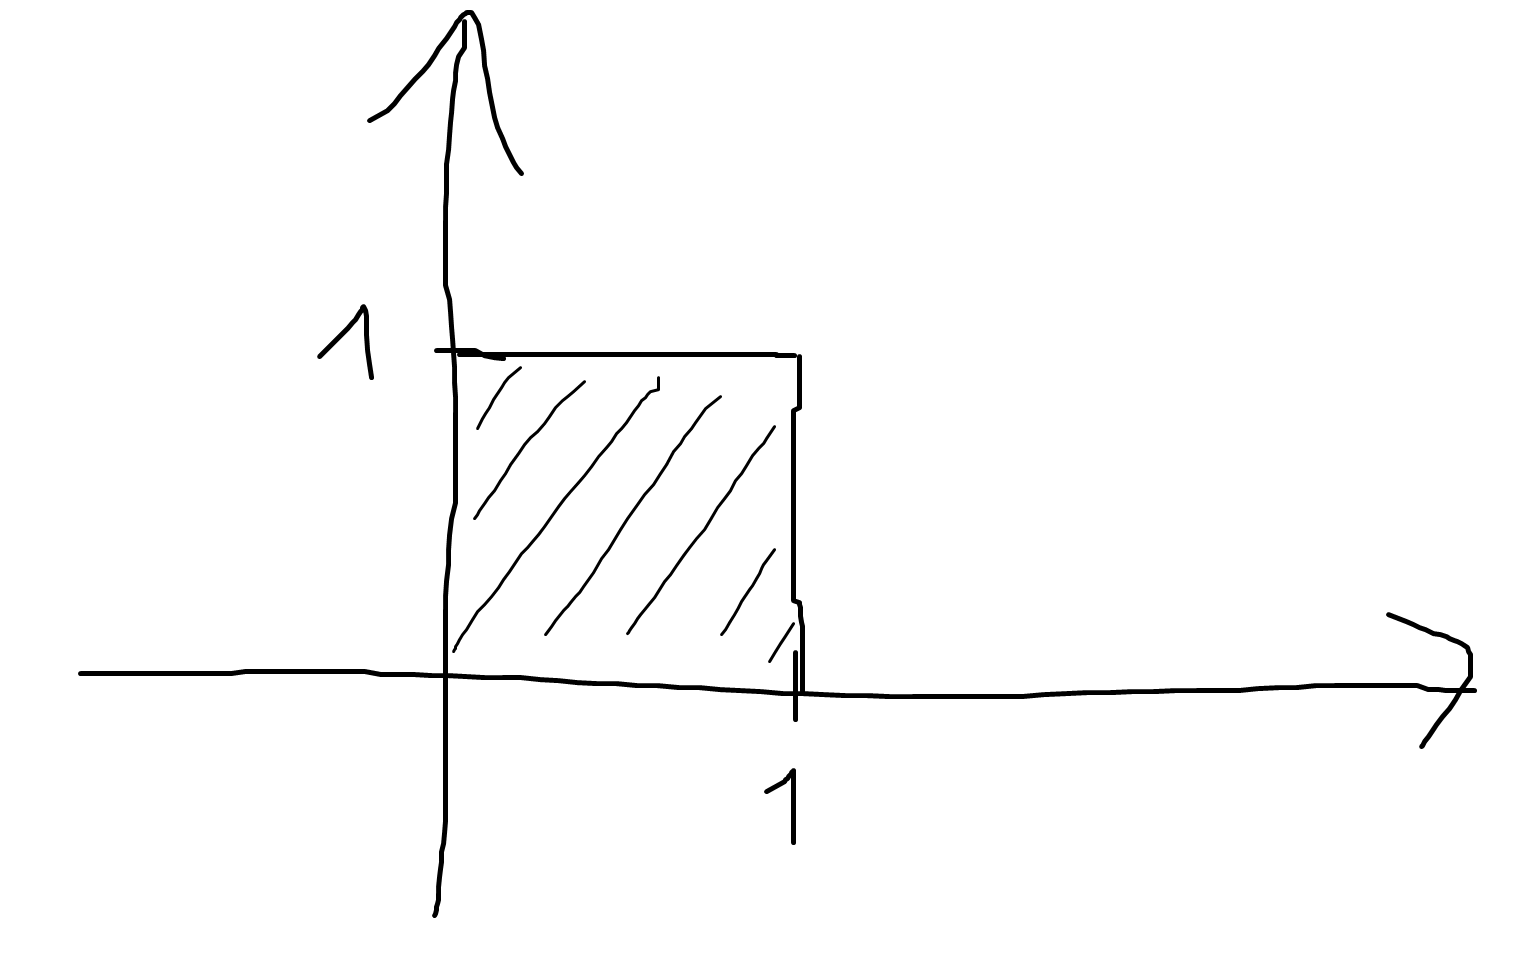
\includegraphics[width=4cm]{kepek/01.png}
			\caption{}
		\end{figure}
		\[ \tau_n^1:=\left\{ \frac{i}{n}\in\R:\quad i\in\{0,\ldots,n\} \right\}=:\tau_n^2,\quad \tau_n:=\tau_n^1\times\tau_n^2\in\mathcal{F}(T)(n\in\N) \]
		\[ x_i:=\frac{i}{n},\quad y_j:=\frac{j}{n}\quad (i,j\in\{0,\ldots,n\}),\quad T_{ij}:=[x_{i-1},x_i]\times[y_{j-1},y_j] \quad (i,j\in\{1,\ldots,n\}) \]
		\[\Rightarrow\quad \mu(T_{ij})=(x_i-x_{i-1})(y_j-y_{j-1})=\left(\frac{1}{n}-\frac{i-1}{n}\right)\left(\frac{j}{n}-\frac{j-1}{n}\right)=\frac{1}{n^2}\]
		\[ s(f,\tau)=\sum_{i,j=1}^n\inf\{ f(r)\in\R:\quad r\in T_{ij} \}\cdot\mu (T_{ij})=\sum_{i,j=1}^nx_{i-1}y_{j-1}\cdot\frac{1}{n^2}=\frac{1}{n^2}\sum_{i,j=1}^n\frac{i-1}{n}\cdot\frac{j-1}{n}=\]
		\[=\frac{1}{n^4}\cdot\left(\sum_{i=1}^n(i-1)\right)\left(\sum_{j=1}^n(j-1)\right)=\frac{1}{n^4}\cdot\frac{(n-1)n}{2}\cdot\frac{(n-1)n}{2}=\frac{1}{4}\left(1-\frac{1}{n}\right)^2 \]
		\[ S(f,\tau_1)=\sum_{i,j=1}^n\sup\{ f(r)\in\R:\quad r\in T{ij} \}\mu(T_{ij})=\sum_{i,j=1}^nx_iy_i\cdot\frac{1}{n^2}=\frac{1}{n^2}\left(\sum_{i=1}^n\right)\left(\sum_{j=1}^nj\right)=\]
		\[=\frac{1}{n^2}\cdot\frac{n(n+1)}{2}\cdot\frac{n(n+1)}{2}=\frac{1}{4}\left(1+\frac{1}{n}\right)^2 \]
		\[ \lim_{n\to\infty}(s(f,\tau_n))=\frac{1}{4}=\lim_{n\to\infty}(S(f,\tau_n)) \]
	\end{task}
%	\begin{theorem}
%		(állítás)
%		
%		\[\sup\{ s(f,\tau)\in\R:\quad \tau\in\mathcal{F}(T)\}=\frac{1}{4}\]
%		
%		\textit{Bizonyítás:} 
%		
%		1. lépés: $\forall \tau, \mu\in \mathcal{F}(T)$ \[s(f,\tau)\leq S(f,\mu)\quad \Rightarrow\quad s(f,\tau)\leq\inf\{ s(f,\tau_n)\in\R: \quad n\in\N \}=\lim(S(f,\tau_n))=\frac{1}{4}\]
%		2. lépés: 
%		
%		%TODO bepótolni
%	\end{theorem}
%	\begin{theorem}
%		$T\subset\R^N$ tégla, $f:T\to\R$ korlátos függvény %TODO pótolni
%	\end{theorem}
\end{document}